\section{Language Models}

A vector space model (VSM) represents words as sequences of vectors (Ibrahim, 2019). 

A language model is a kind of vector space model that takes as input a sequence of word vectors and outputs a sequence of predicted word vectors by learning a probability distribution over words in a vocabulary. In representation terms, the "vector representation of a word depends on the context vector representation" (Ibrahim, 2019).

Many tasks such as machine tranaslation, spell correction, text summarization, question answering, and sentiment analysis all use language models to convert text into machine-interpretable language (Chromiak, 2017). 

Intuitively, language models predict words in a blank. For instance, given the following context: "The $\_\_\_$ sat on the mat" where $\_\_\_$ is the word to predict, a language model might suggest the word "cat" should fill the blank a certain percentage of the time and the word "dog" would fill the blank with lower probability (Kurita, 2019). 

Formally, language models work by computing the conditional probability of a word $w_t$ given a context, such as its previous $n-1$ words, where the probability is: $P(w_t | w_{t-1}, ..., w_{t-n+1})$ (Ruder, 2016). Chromiak adds that the probability chain rule is the main tool used to find the joint probability of a word sequence. For events A and B, the probability chain rule states:
$$
P(A | B) = \frac{P(A \cap B)} {P(B)}
$$
which lends the following formula for a set of $T$ word tokens $w_1, ..., w_T$ from a sentence $S$: 
$$
\begin{array}{ll}
P(S)
&= P(w_1, ..., w_T)  \\
&= P(w_1) \cdot P(w_2 | w_1) \cdot ... \cdot P(w_n | w_1, ..., w_{T-1}) \\
&= \prod_{t=1}^T P(w_t | w_1, ..., w_{t-1}) \\
\end{array}
$$
Typically, the \textbf{Markov Assumption}, which states that the probability of a word depends only on its previous word, is used to reduce context history and thus intake of model data. Thus the joint probability is estimated using the $n$ previous words of the current word $w_t$:
$$
P(w_1, ..., w_T) \approx \prod_{t=1}^T P(w_t | w_{t-1}, ..., w_{t-n+1})
$$

There are several kinds of language models. 

\subsection{n-gram Language Model}

An n-gram is a sequence of $n$ words. The n-gram language model is one of the simplest models that assigns probabilities to sentences and word sequences. It calculates a word's probability based on the frequencies of its constituent n-grams, taking just the preceding $n-1$ words as context instead of the entire corpus (Ruder, 2016): 
$$
P(w_t | w_{t-1}, ..., w_{t-n+1}) = \frac {count(w_{t-n+1},...,w_{t-1},w_t)} {count(w_{t-n+1},...,w_{t-1})}
$$

\subsection{Neural Network Language Model}

A neural network calculates the probability of word vector $w_t$ using a softmax layer: 
$$
P(w_t | w_{t-1}, ..., w_{t-n+1}) = \frac {\exp{(h^T \cdot v_{w_t}') }} {\sum{w_i \in V} \exp{(h^T \cdot v_{w_i}') }}
$$
where $V = $ vocabulary of a corpus, $h = $ output vector of the hidden layer, and $v_w' = $ the output embedding of word $w$. 

\subsection{Forward Language Model}

\subsection{Backward Language Model}

\subsection{Bidirectional Language Model}

\begin{figure}[h]
\centering
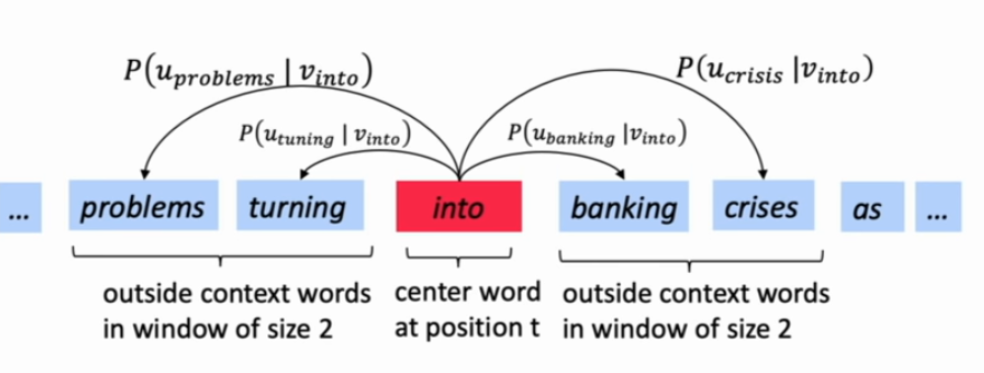
\includegraphics[width=0.8\textwidth]{bidirectional_languagemodel_banking.png}
\caption{Example Bidirectional Language Model. From \emph{Word2Vec Overview With Vectors}, by CS224n: Natural Language Processing with Deep Learning (Stanford), 2018. \url{https://sangminwoo.github.io/2019-08-28-cs224n-lec1/}. Copyright n.d. by n.d.}
\end{figure}



--------------------------

\subsection{Word Embedding Representations: Count-Based vs. Context-Based}

LILIAN WENG: https://hyp.is/dKRaygVnEeqRaI-_7zzFtQ/lilianweng.github.io/lil-log/2017/10/15/learning-word-embedding.html
"There are two main approaches for learning word embedding, both relying on the contextual knowledge.

Count-based: The first one is unsupervised, based on matrix factorization of a global word co-occurrence matrix. Raw co-occurrence counts do not work well, so we want to do smart things on top.
Context-based: The second approach is supervised. Given a local context, we want to design a model to predict the target words and in the meantime, this model learns the efficient word embedding representation."


One way to convert human text into machine-interpretable data is to use a one-hot encoding. Essentially, each distinct word stands for one dimension of the resulting vector a

----------------------------

